\documentclass[11pt, oneside]{article} 
\usepackage{geometry}
\geometry{letterpaper} 
\usepackage{graphicx}
	
\usepackage{amssymb}
\usepackage{amsmath}
\usepackage{parskip}
\usepackage{color}
\usepackage{hyperref}

\graphicspath{{/Users/telliott/Github/precalculus/fig/}}
% \begin{center} \includegraphics [scale=0.4] {gauss3.png} \end{center}

\title{Lines and angles}
\date{}

\begin{document}
\maketitle
\Large

\subsection*{Euclid and the postulates}
Greek geometry starts hundreds of years before Euclid, who was a contemporary of Alexander the Great (356-323 BC).  

We know that Euclid lived after Plato (died 347 BC), and before Archimedes (born 287 BC).  Except that he worked in Alexandria, all other details of his life and death are shrouded in mystery.

After more than 2000 years, Euclid's book \emph{Elements} is still an excellent place to begin surveying the foundations of geometry.  It is a textbook, an organized collection of everything that a well-educated student was expected to know about the subject at the time.

\begin{center} 
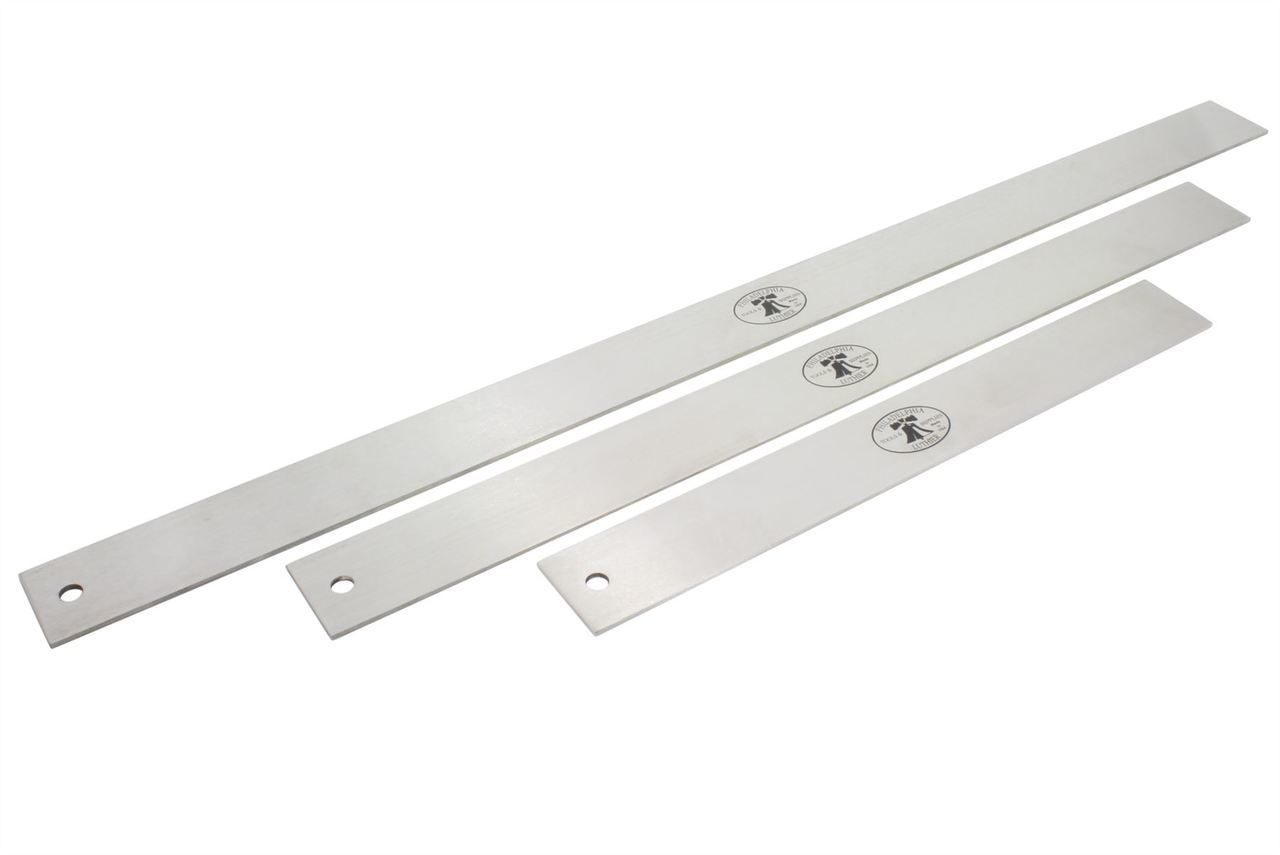
\includegraphics [scale=0.2] {straightedge.png} 
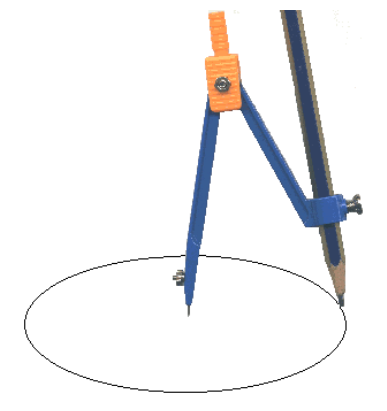
\includegraphics [scale=0.3] {compass.png} 
\end{center}

This book of consists of \emph{propositions}, which include constructions (geometric figures) drawn with a pencil on a piece of paper, using a straight-edge or a compass or both.  Often proofs of propositions build on previous items in the book.  

Euclid does not prove everything.  Statements which are assumed to be true are postulates and axioms.

Here are Euclid's first three postulates:

$\bullet$  A straight line segment can be drawn joining any two points.

\begin{center} 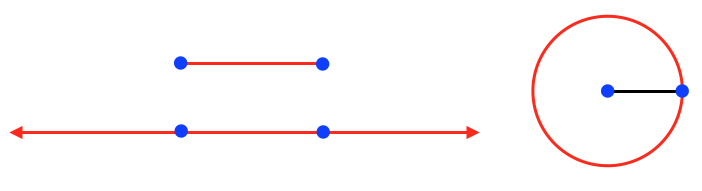
\includegraphics [scale=0.4] {postulates.png} \end{center}

$\bullet$   Any straight line segment can be extended indefinitely in a straight line.

$\bullet$   Given any straight line segment, a circle can be drawn having the segment as the radius and one endpoint as the center.

Let us assume these as well.  We will use them often.

We finesse the difficulty in defining what is meant by \emph{straight} in the real world.  If you've ever done any carpentry, you know that unknown edges are determined to be straight by comparison with another edge known to be straight.

In geometry, we use an imaginary perfect straight-edge to draw a straight line as "the shortest distance between two points".

\subsection*{measure of an angle}

Consider the diagram below. One line segment is drawn crossing a second one, forming their \emph{intersection}

\begin{center} 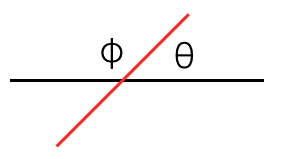
\includegraphics [scale=0.4] {lines_angles_0.png} \end{center}

Two angles are labeled.  One, $\phi$, is larger than the other one, $\theta$.  
\[ \phi > \theta \]

Writing the statement $\phi > \theta$ is easy, but the implication is that we have some way of taking the \emph{measure} of an angle.  We can't just rely on a picture.

Our answer is to construct a circle around the central point, and call the distance along the circumference between the points where the lines cross the circle, the measure of the angle.

If that distance along the edge is larger for $\angle \phi$ than for $\angle \theta$, then $\phi > \theta$.  In the left panel, the arc between $Q$ and $R$ (call it arc $QR$) is larger than arc $PQ$.

\begin{center} 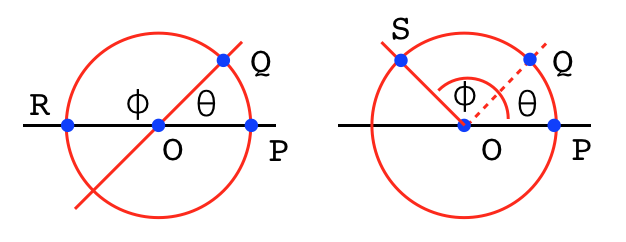
\includegraphics [scale=0.4] {lines_angles_00.png} \end{center}

We don't need to actually measure the arc.  

Instead we can use a standard compass to lay off the linear distance from $Q$ to $R$ starting from $P$ (right panel).  Since $S$ is further around the circle from $P$ than $Q$ is, $\phi > \theta$.

(This doesn't work very well as $S$ approaches the diameter through $O$ and $P$, but we could add the distance in two parts and that would be fine).  

Let us call angles formed on the same side of a line, \emph{supplementary} angles (also sometimes called adjacent angles).

\begin{center} 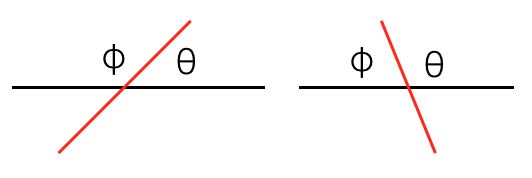
\includegraphics [scale=0.4] {lines_angles_1.png} \end{center}

$\circ$ \ On the left, one of the angles, $\phi$, is larger than the other one, $\theta$.  

$\circ$ \ On the right, we have $\phi < \theta$.  

$\circ$ \ The third possibility is that $\theta = \phi$.

\subsection*{right angles}

Euclid's fourth postulate is:

$\bullet$  \ All right angles are congruent, that is, equal to each other.

The definition of a right angle is that 

$\bullet$ \ if two supplementary angles are equal, then they are both right angles.  

\begin{center} 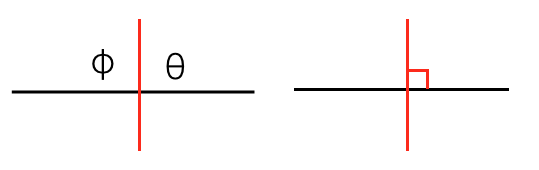
\includegraphics [scale=0.4] {lines_angles_2.png} \end{center}

A right angle is frequently designated by drawing a small square, as seen in the right panel above.

Regardless of the relation between $\theta$ and $\phi$:

$\bullet$ \ the sum of two supplementary angles is equal to two right angles.

A corollary is that the sum of all the angles on one side of a line (at a given point), is equal to two right angles.

\begin{center} 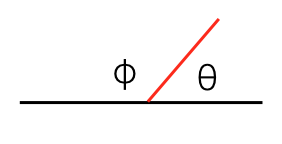
\includegraphics [scale=0.35] {lines_angles_5.png} \end{center}

This is simply a matter of subtraction.  If the sum of all the angles at a point is equal to four right angles, then the sum of the angles on each side of a line through that point is equal to two right angles.

The convention that there are $360^{\circ}$ total in a circle dates to the time of the Babylonians (c. 2400 BC).

In degrees, a right angle is $90^{\circ}$ and two supplementary angles measure $180^{\circ}$.  

There is nothing particularly special about using $90^{\circ}$ as the measure of a right angle, or $360^{\circ}$ for one whole turn.  Well, there is one thing:  there are \emph{approximately} 360 days in a year, which marks the sun's track across the sky.  

In his book, \emph{Measurement}, Lockhart adopts the convention that a whole turn is equal to $1$.  

We'll just mention here that one whole turn can be defined using a different unit of measure as $2 \pi$ \emph{radians}, and that convention turns out to be quite important for calculus.

\begin{center} 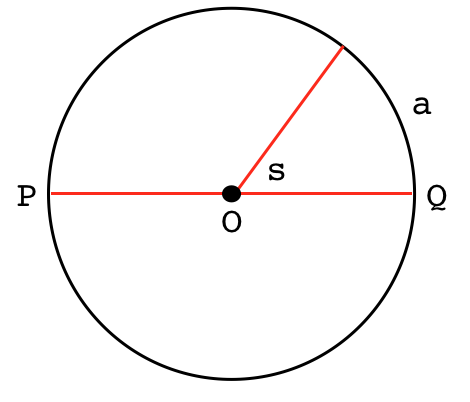
\includegraphics [scale=0.35] {arcs11.png} \end{center}

In the figure above, we \emph{define} the measure of the angle $s$ to be equal to the arc it sweeps out or subtends, $a$, in a circle of radius $1$, a \emph{unit} circle.  Angles are not lengths, but numerically, the measure of the angle is the measure of the arc.

\subsection*{vertical angle theorem}

Now, consider those angles lying below the horizontal:

\begin{center} 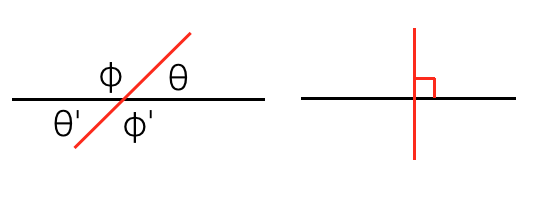
\includegraphics [scale=0.4] {lines_angles_3.png} \end{center}

We said that the sum of the two angles $\phi + \theta$ is equal to two right angles, but so are the sums $\theta' + \phi$ and $\theta + \phi'$, for the same reason.  As a result

\[ \phi + \theta = \theta + \phi' \]
We conclude that 
\[ \phi = \phi' \]
and
\[ \theta = \theta' \]

$\bullet$ \ This is the \emph{vertical angle theorem}.

\begin{center} 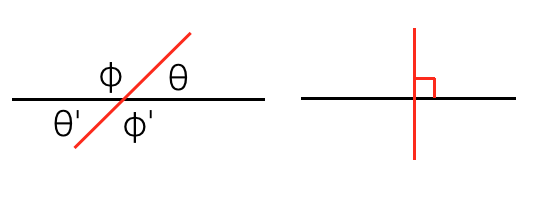
\includegraphics [scale=0.4] {lines_angles_3.png} \end{center}

On the right, if any one of the angles where two lines cross is a right angle, then all four are right angles.

Finally, the idea is generalizable to more than just two angles.  In the figure below
\begin{center} 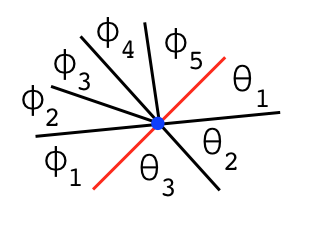
\includegraphics [scale=0.4] {lines_angles_000.png} \end{center}

\[ s = \phi_1 + \phi_2 + \phi_3 + \phi_4 + \phi_5 \]
\[ t = \theta_1 + \theta_2 + \theta_3 \]
\[ s = t = \pi \]
\[ s + t = 2 \pi \]

Both sums are equal to two right angles.

$\bullet$ \ when one or more lines cross a given line at the same point, the angles formed on one side of the given line have a total measure equal to two right angles.

$\bullet$ \ the total of all the angles formed at that point is equal to four right angles.

\subsection*{parallel postulate}

So far, all this seems rather obvious.  The fifth and final postulate is more subtle.

In the figure, line $1$ and line $2$ are parallel, \emph{if and only if}
\[ A + C = B + D = 180 = 2 \ \text{right angles} \]

\begin{center} 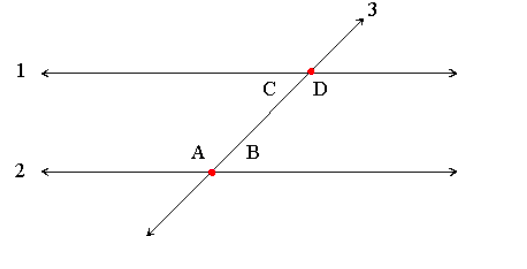
\includegraphics [scale=0.5] {alternate_interior_angles.png} \end{center}

$\bullet$   If two lines are drawn which intersect a third in such a way that the sum of the inner angles on one side is less than two right angles, then the two lines inevitably must intersect each other on that side if extended far enough.

This postulate is equivalent to what is known as the parallel postulate.

\url{http://mathworld.wolfram.com/EuclidsPostulates.html}

\subsection*{alternate interior angles}

We come to a very important theorem.

In the figure above, the supplementary angles $A + B$ also add up to $180^{\circ}$. So
\[ A + B = 180 = A + C \]
and then
\[ B = C \]

This is called the theorem on \emph{alternate interior angles} between two parallel lines.

\begin{center} 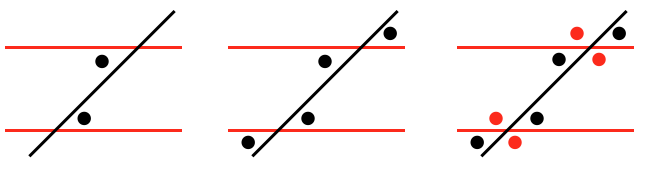
\includegraphics [scale=0.4] {lines_angles_4.png} \end{center}

In the figure above (left panel), we're given that the two horizontal lines are parallel.

The indicated angles are equal because they are alternate interior angles of two parallel lines (parallel postulate).  

In the middle panel, two additional equalities are established by the vertical angle theorem.  Then on the right, we use the supplementary angle theorem.

Note that the conclusions for the angles marked with a red dot are themselves consistent with the three theorems:  supplementary and vertical angles and alternate interior angles.

\subsection*{summary}

Make sure you learn and understand each of these theorems:

$\bullet$ \ the sum of two supplementary angles is equal to two right angles.

$\bullet$ \ vertical angles are equal

$\bullet$ \ alternate interior angles of two parallel lines are equal

There is one more in this chapter, coming below:

$\bullet$ \ the sum of angles in a triangle  is equal to two right angles.

Another point to remember:  these are two-way, \emph{if and only if} theorems.  

So for example, if the two alternate interior angles of a traversal are equal, the two lines are parallel.

\subsection*{flat geometry}

Adoption of the parallel postulate is a choice.  The definition works for geometry in the flat plane, but not on a curved surface like the earth's surface.  That's a familiar situation where our postulate is not appropriate.

Then, two adjacent lines of longitude can be drawn so as to cross the equator at right angles, and the lines are parallel there, but they will meet (intersect) at the poles.  

\begin{center} 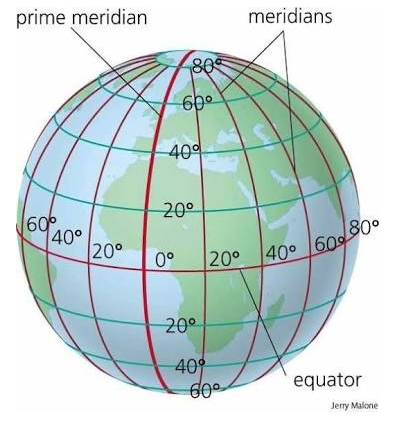
\includegraphics [scale=0.5] {lat_long.png} \end{center}

The parallel postulate only holds for geometry on a \emph{flat} surface.

\subsection*{axioms}

Euclid also lists five axioms, things which are assumed.  Here are two examples:

$\bullet$   Things that are equal to the same thing are also equal to one another.

$\bullet$   If equals are added to equals, then the wholes are equal.

These seem quite reasonable.

We will see how to proceed from the postulates and axioms to various proofs.  Given these \emph{assumptions}, we can prove theorems that must be true.

\subsection*{Thales}
William Dunham has written a lot about the history of mathematics in Greece, starting with Thales (624-546 BC), who was from a Greek town called Miletus on the coast of Asia Minor (modern Turkey).  He lived long before Euclid (about 300 years before, 600 BC).  Although none of his writing survives, it is believed that Thales proved several early theorems including the ones we saw above. 

A very important theorem attributed to Thales is the following:

$\bullet$  The angle sum of a triangle is equal to two right angles.
\begin{center} 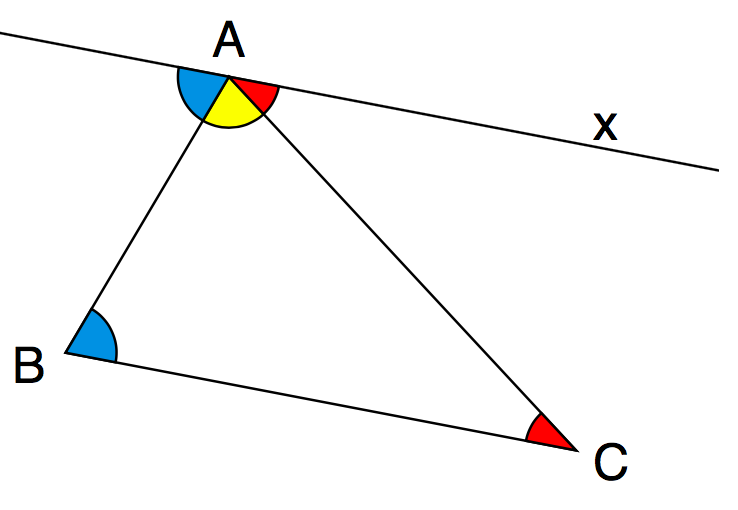
\includegraphics [scale=0.3] {triangle_sum_angles.png} \end{center}

This theorem depends on the ideas we developed above.  

Proof.

Draw a line segment through $A$ parallel to $BC$.  Now, use alternate interior angles and follow the colors to the result.

$\square$

We will see one last theorem ascribed to Thales (it is actually called Thales' theorem), in the next chapter.  It is a result about isosceles triangles (two sides equal).

\subsection*{another proof}
Here is a different proof of the theorem on the sum of angles in a triangle adding to 180 degrees.  It never hurts to re-prove things by a different method.  This serves as a check on both the result and the methods.

Imagine walking around the perimeter of a triangle in the counter-clockwise direction.  At each vertex we turn left by a certain number of degrees, $\theta$, called the exterior angle.  After passing through all three vertices, we must end up facing in the same direction as we started.

The sum of the exterior angles is $360^\circ$.

\begin{center} 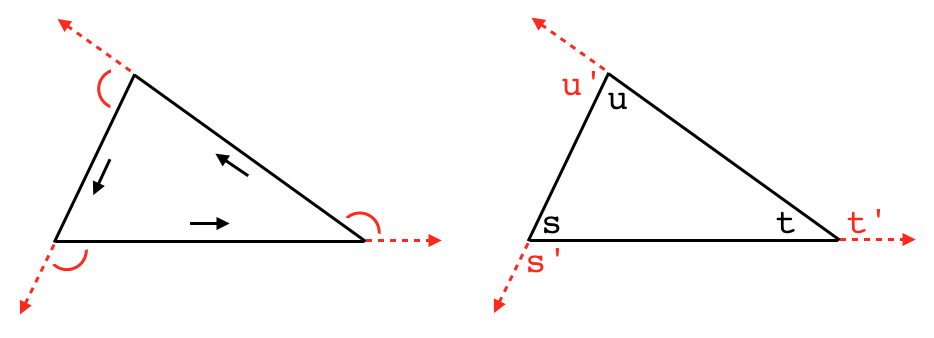
\includegraphics [scale=0.4] {lines_angles_trisum.png} \end{center}

\[ s' + t' + u' = 360 \]

In addition, for each vertex, the interior angle plus the exterior angle add up to $180$ degrees.  If we add all three pairs, we obtain
\[ (s + s') + (t + t') + (u + u') \]
\[ 180 + 180 + 180 = 540 \]
By subtraction
\[ s + t + u = 180 \]

$\square$

\end{document}